\section{Introduction}
\label{sec:introduction}

The use of deep learning models has risen in many applications. With it, so too has the desire to understand why these models make certain predictions. These models are often referred to as ``opaque'', as it is difficult to discern the reasoning behind their predictions \citep{marcus2018deep}. Additionally, deep learning models can inadvertently learn and perpetuate biases found in their training data \citep{sap2019risk}. To create fair and trustworthy algorithms, it is essential to be able to explain a model's output \citep{das2020opportunities}. 

Some examples of the methods proposed to explain neural networks include Gradient SHAP \cite{lundberg2017unified}, Integrated Gradients  \citep{sundararajan2017axiomatic} and  \citep{kapishnikov2021guided}.

Significant effort has been dedicated to designing explanation methods that satisfy certain desirable axioms. This is due to the lack of ground truth for evaluating them. The axioms can ensure that the explanations are principled. One of the most successful axiomatic methods is Integrated Gradients (IG) \citep{sundararajan2017axiomatic}. Consider a function $f : R^n \to R$, representing the neural network and an input vector $\textbf{x} \in R^n$. Furthermore, consider a baseline input vector $\overline{\textbf{x}} \in R^n$ (typically chosen such that the network gives baseline a near zero score). IG explains the network by quantifying how much of the difference $f(\textbf{x}) - f(\overline{\textbf{x}})$ can be attributed to the $i$th dimension of $\textbf{x}$, $\textbf{x}_i$.

Integrated Gradient gives attribution $IG_i$ to the $i$th dimension of the input by solving the following path integral
\begin{equation}
IG_i(\textbf{x}) = (\textbf{x}_i - \overline{\textbf{x}}_i) \int_0^1 \frac{\partial f(\gamma(t))}{\partial \textbf{x}_i} dt, \label{eq:igi}
\end{equation}
where $\gamma(t) = \overline{\textbf{x}} + t(\textbf{x} - \overline{\textbf{x}})$ is a straight path from the baseline to input. The claim of the creators of IG is that Eq. \ref{eq:igi} tells us how the model got from predicting essentially nothing at $\overline{\textbf{x}}$ to giving the prediction at $\textbf{x}$. Considering gradients represent the rate of change of functions, the above expression should tell us how scaling each feature along the path affects the increase in the network score for the predicted class.

\begin{figure}[t!]
	\begin{center}
		\centerline{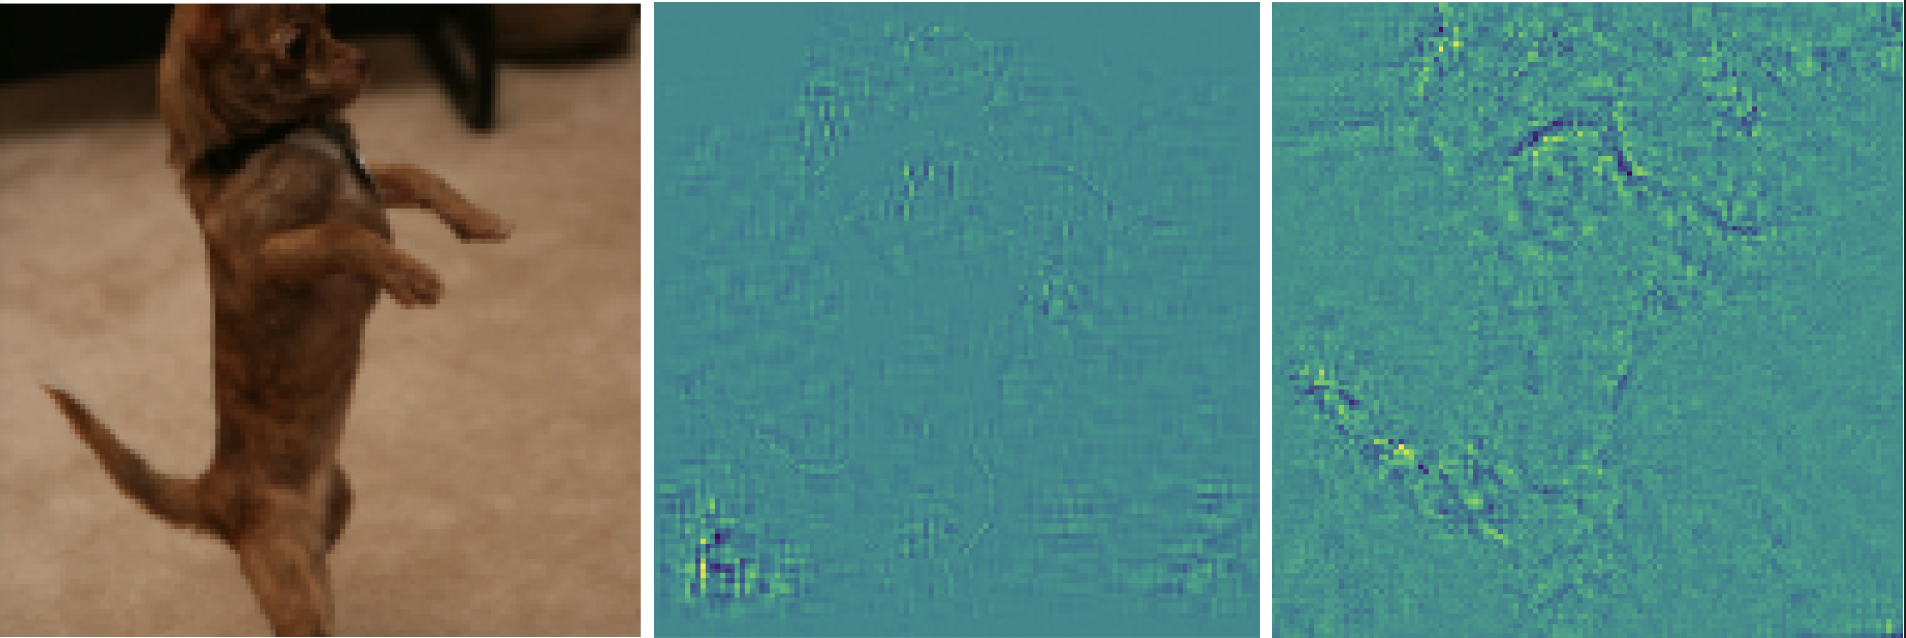
\includegraphics[width=0.95\columnwidth]{figures/voc_compare.png}}
		\caption{Comparison of attributions generated by Integrated Gradients (middle image) and Geodesic Integrated Gradients (right image). Integrated Gradients follow straight paths in Euclidean space, which can result in misleading attributions. In contrast, Geodesic Integrated Gradients integrate along geodesic paths on a Riemannian manifold defined by the model, correcting the misattributions due to poor alignment with the model's gradient landscape.}
		\label{fig:duck}
	\end{center}
	\vskip -0.3in
\end{figure}

In this paper, we demonstrate that defining attributions along straight paths in Euclidean space can lead to flawed explanations. We examine the consequences of these issues through examples in computer vision, as shown in Fig. \ref{fig:duck}, along with simpler, illustrative cases in Fig. \ref{fig:ig}. To address these challenges, we introduce \textbf{Geodesic Integrated Gradients} \footnote{The code for the attribution methods and reproducing the experiments is provided on \href{https://github.com/sina-salek/geodesic-ig}{https://github.com/sina-salek/geodesic-ig}}, a generalisation of IG that replaces straight paths with geodesic ones. These geodesics are defined on a Riemannian manifold, characterised by the model's input space and a metric induced by the model's gradients. This approach mitigates the identified pitfalls while retaining all the axioms of IG.

Before making the case for our Geodesic Integrated Gradient, let us first show an example of an artefact that can arise from choosing straight paths, generating explanations which do not reflect the true behaviour of a model. 

We highlight this issue on a half-moons classification task. We train a simple multi-layer perceptron (MLP) with 3 layers, ReLU activations and a cross-entropy loss to distinguish the upper moon from the lower one. The cross-entropy is split into a final log-softmax activation and a negative log-likelihood loss, so that we can explain probabilities.

We now compute Integrated Gradients, Eq. \ref{eq:igi}, for this model on the test data. Let us consider a baseline and input pair, such that the baseline is outside of either half-moon, for example at (-0.5, -0.5). This is a good choice of baseline, since network should assign near-zero score to it. Let us call the feature in the vertical axis the $1$st component of $x$. In Fig. \ref{fig:ig} we illustrate the attribution of this feature, $IG_1(\textbf{x})$, for each point using the colour map. One should expect to see all the points sufficiently above the decision boundary to receive equally high attributions. Intuitively, this is expected, because if a point is above the decision boundary, its $x_1$ component is an important factor in the classification. However, for a model that is very skillful at the classification task, since the point is significantly above the decision boundary, going slightly down should not make any difference. Because in such a model's score should not change significantly anywhere other than near the decision boundary. However, we can see in Fig. \ref{fig:ig} that some points on the upper moon receive much higher $x_1$-attribution than others. These are points such that a straight line from the baseline to them mostly falls on high gradient regions. This does not reflect the model's behaviour. A similar point could be made about the horizontal axis. This is in contrast with Fig. \ref{fig:ig}, where we show our method gives equally high attribution to all points sufficiently above the decision boundary, with different shades for the points closer to the boundary in $x_1$ direction. In Section \ref{subsec:half-moons} we present the details of how our method that achieves the results presented in this figure.

\begin{figure}[t!]
\vskip -0.1in
\begin{center}
\centerline{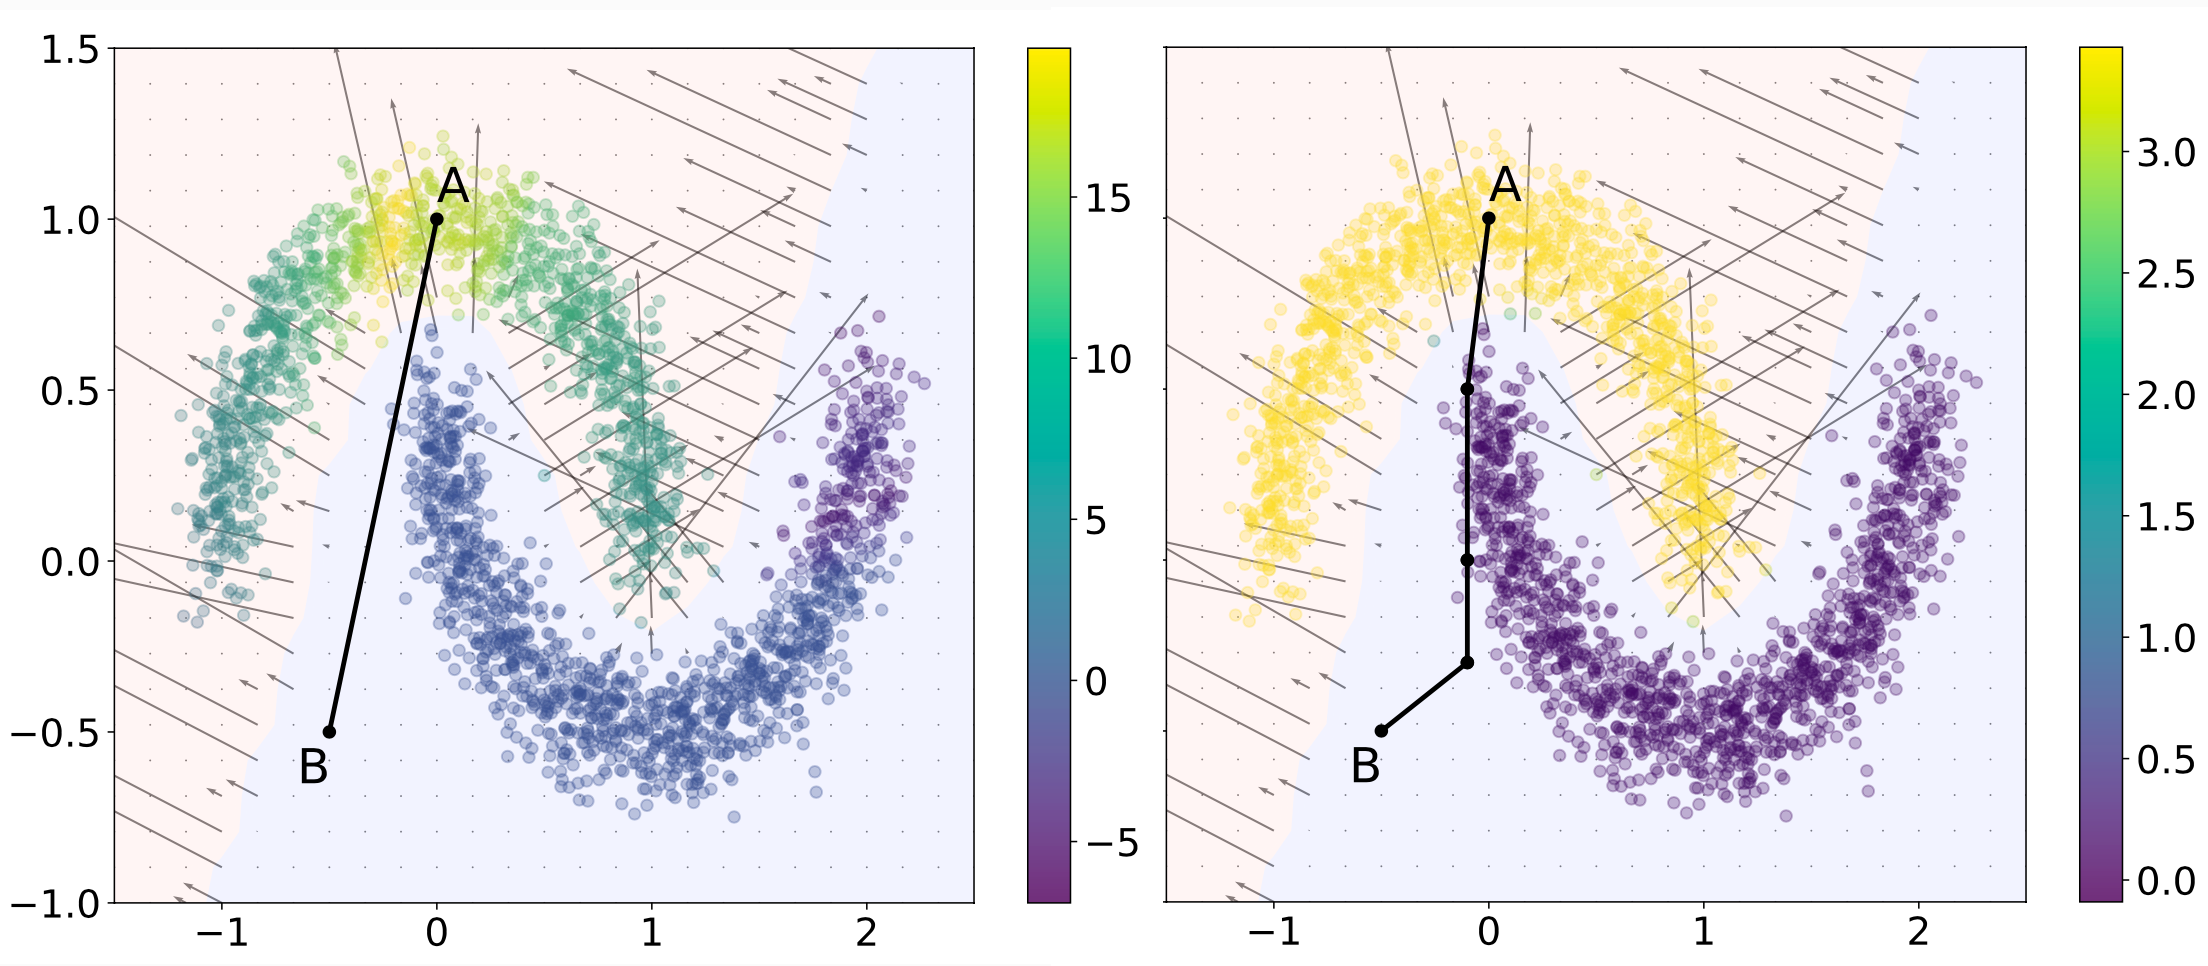
\includegraphics[width=\columnwidth]{figures/half_moons_y.png}}
\vskip -0.2in

\caption{\textbf{Integrated Gradients (IG) attributions (left) vs. Geodesic IG (right).} The colour map shows feature attributions on the vertical axis, with $(-0.5, -0.5)$ (point B) as the baseline. In IG, points near $A$ are over-attributed due to the straight path crossing high-gradient regions near the decision boundary (gray arrows). Geodesic IG avoids this issue by following geodesic paths, providing more accurate attributions.}
\label{fig:ig}
\end{center}
\vskip -0.2in
\end{figure}

\begin{figure}[!hbp]
	\vskip 0.2in
	\begin{center}
		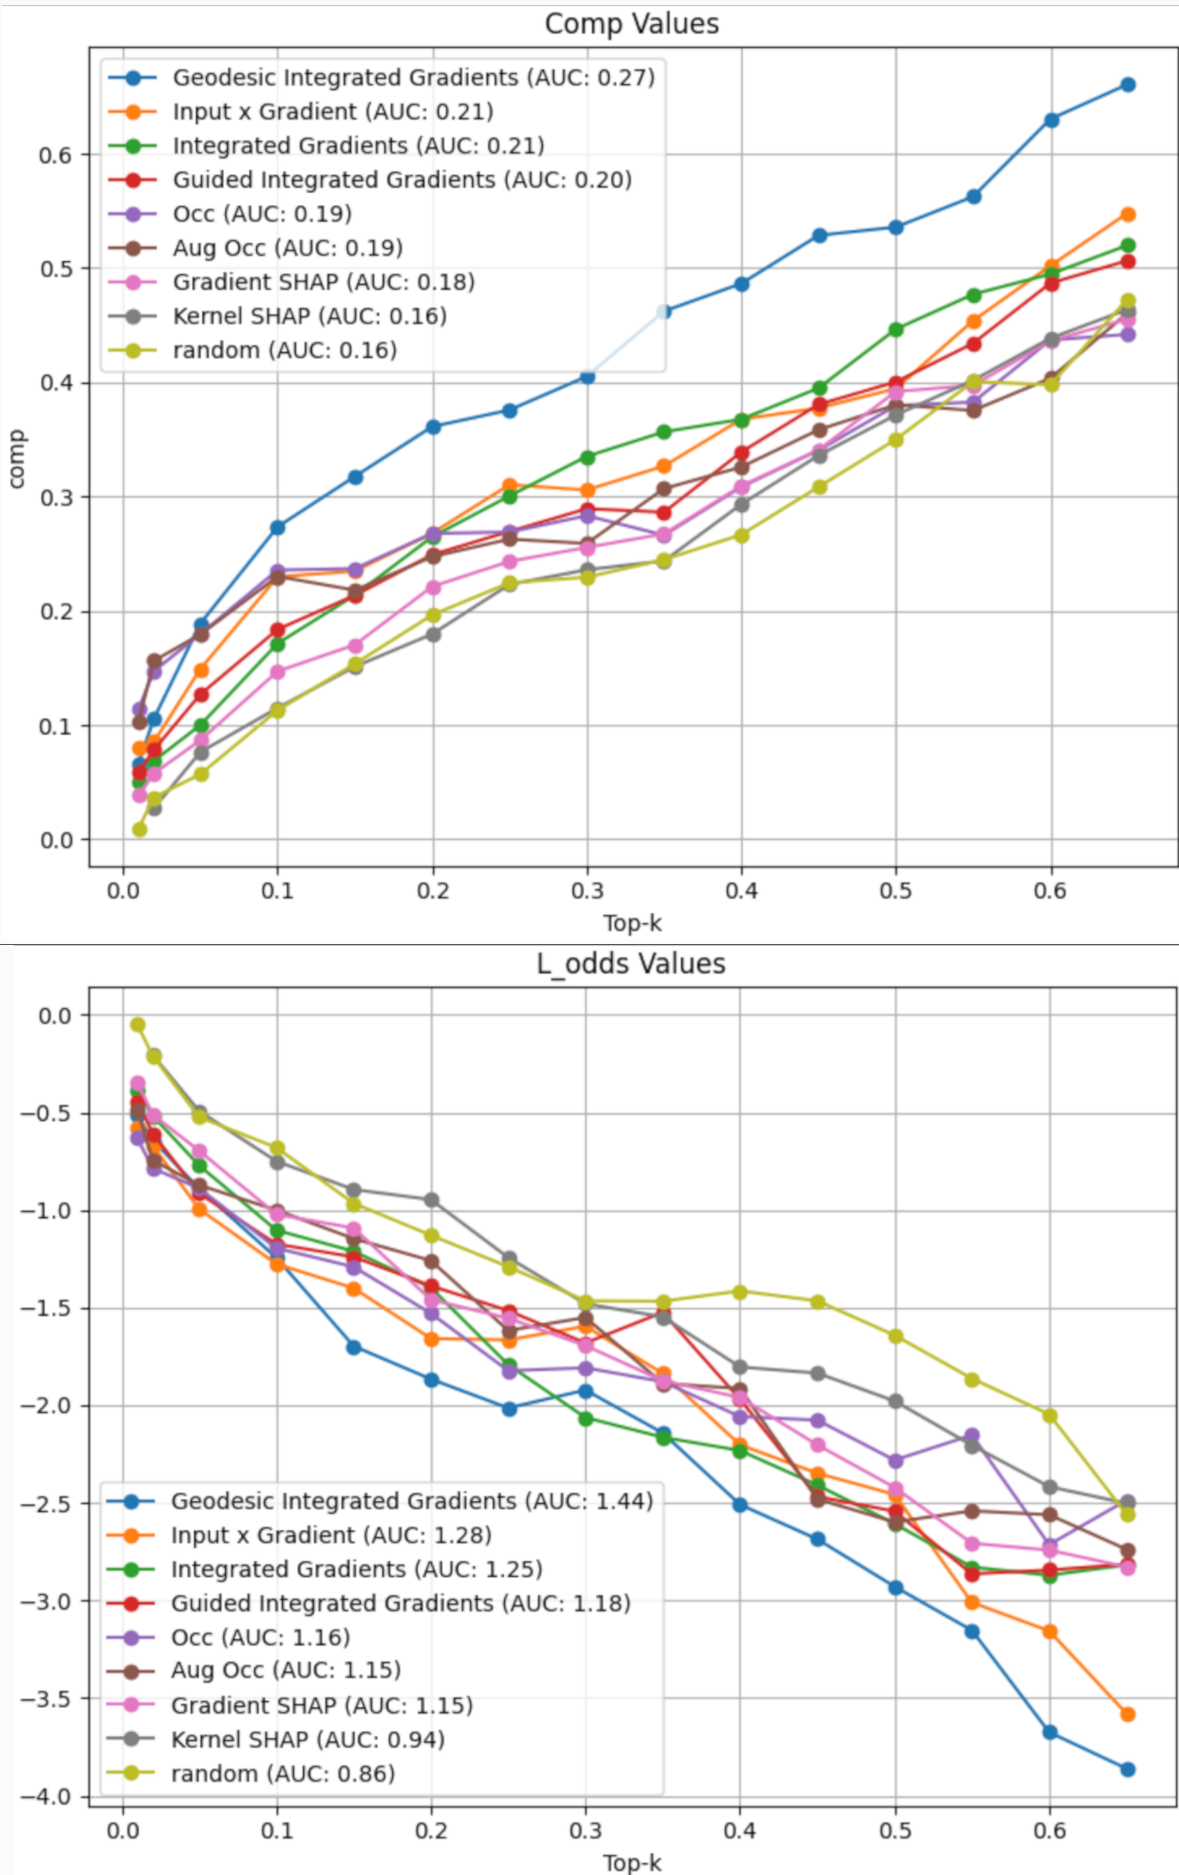
\includegraphics[width=0.85\columnwidth]{figures/voc_metrics_vertical.png}
		\caption{ \textbf{Metrics Comparison.} We use a ConNext model for classification of images from the VOC dataset. The horizontal axis represents the top $k\%$ (in absolute value) of features being selected. The top plot, \textit{Comprehensiveness}, shows the average change in the predicted class probability of compared to the original image (higher is better). The bottom plot displays the negative logarithmic probabilities of the predicted class relative to the original (lower is better). In both cases, the results are summarised using AUC, where higher values are better for both.}
		\label{fig:voc_metrics}
	\end{center}
	\vskip -0.2in
\end{figure}

Before giving the formal method in section \ref{sec:method}, let us discuss the intuition behind our Geodesic IG. We want the path in Eq. \ref{eq:igi} to be such that it avoids regions with high model gradient. This is because failing to do so would superficially increase the result of the integral, leading to the types of artefacts illustrated in Fig. \ref{fig:ig}. Therefore, we should try to find the path of least resistance, as this is the path that avoids steep gradients as much as possible. As we shall see in section \ref{sec:method}, the input space can be viewed as a Riemannian manifold with a metric derived from the model gradients. The path of least resistance between a chosen baseline and input, therefore, is the geodesic path between the two points.

In Section \ref{sec:method}, we present two methods for approximating the geodesic path between two points on a manifold. The first method, based on $k$-nearest neighbors ($k$NN), is designed for simpler manifolds, while the second method, utilising Stochastic Variational Inference, is suited for more complex manifolds. We further demonstrate that Geodesic IG adheres to all the axioms of Integrated Gradients.


In Section \ref{sec:experiments}, we demonstrate the effectiveness of the Geodesic IG method on the real-world Pascal VOC 2012 dataset \citep{pascal-voc-2012}. Our results outperform existing methods, as we evaluate using two metrics. We preview the results of this experiment in Fig. \ref{fig:voc_metrics}.

Section \ref{sec:related_work} reviews related work, including the comparison of Geodesic IG with other methods that attempt to overcome the shortcomings of Integrated Gradients.